\chapter{Testing}
\label{chap:testing}

This chapter outlines the process of testing with React.js and Go. The chapter will also cover the use of Postman for API testing \see{testing:postman} and Chrome/React Developer Tools for debugging and testing in the browser \see{testing:chrome-dev}.

\section{Unit Testing}
\label{testing:unit}

Unit testing was critical to the development and functionality of the artefact. They were used primarily to test the core logic of the front and back end. These tests culminate to ensure that the end product is functioning as expected, delivering the complete application that the user expects.

For the Go/Gin backend, the built-in Go test framework was used. For the React.js front, the Jest testing framework was used. The respective plugins were installed in VS Code to allow for easy running and visualisation of the tests \see{fig:unit-tests}.

Multiple tests were written to test the API GET endpoints. The tests were run via the aforementioned VS Code plugin or the terminal using the command `\texttt{go test}'. Using mock data inputs, the tests were written to ensure that the correct JSON object was returned in the correct format to be exploited by the front end. Further testing of the Go API was conducted using Postman, as outlined in Section \see{testing:postman}.

Testing React.js components was a more complex process than writing tests for vanilla JavaScript. As the tests were required to be on a component-level basis, snapshot testing was used to ensure that the components were rendered correctly. To create a snapshot test, all data required by the component was mocked, including required functions. These functions were mocked using `\texttt{jest.fn}', `\texttt{jest.spyOn}' and `\texttt{mockImplementation}'. MockImplementation was used to mock the ChartJs Chart function, to ensure that the ElevationChart snapshot test was consistent with the actual component. To run the tests, either the command `\texttt{npm test}' or the VS Code plugin was used to run the tests. Further tests were conducted throughout development using the Chrome/React Developer Tools, as outlined in Section \see{testing:chrome-dev}.

Manual unit tests were conducted on the front end to ensure that the components behaved as expected. Some examples of these tests can be seen below. \see{tab:unit-test-results}.

\begin{figure}[!ht]
  \centering
  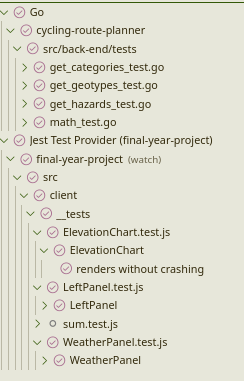
\includegraphics[width=150px]{figures/unit-tests.png}
  \caption{Unit Tests}
  \label{fig:unit-tests}
\end{figure}

\begin{table}[!h]
\caption{Manual Unit Test Results}
\label{tab:unit-test-results}
\renewcommand{\arraystretch}{1.5}
\begin{tabular}{ p{1.85cm} p{10cm}  p{1.85cm} }
\hline
Test Case & Description & Pass?\\
\hline
01 & All components were tested to ensure that they render correctly on load. & Y\\
02 & All components were tested to ensure that they render correctly when changing the route. & Y\\
03 & All components were tested to ensure that they render correctly when zooming/panning the map. & Y\\
04 & All components were tested to ensure that they render correctly when exporting the route. & Y\\
\end{tabular}
\end{table}

\clearpage
\section{Postman}
\label{testing:postman}

Postman was also used extensively through development to test the API. It was used to test the GET and POST endpoints to ensure that the correct data was being returned and that the correct data was being sent to the backend \see{fig:postman-go}. In addition to testing the Go backend, Postman was also used to build and test API requests for Strava, Garmin Connect, Open Weather Map, Foursquare and the Here API \see{fig:postman-external}. This was done to ensure that the API requests were being built correctly before being implemented into the artefact.

\begin{figure}[!ht]
  \centering
  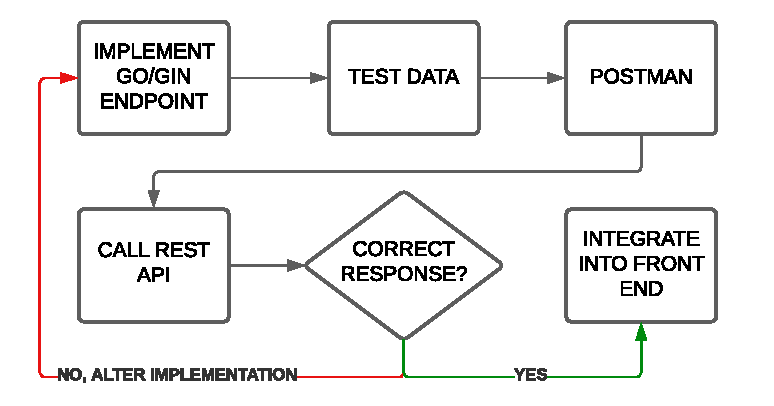
\includegraphics[width=400px]{figures/postman-testing-go.pdf}
  \caption{Postman - Testing Go/Gin APIs}
  \label{fig:postman-go}
\end{figure}

\begin{figure}[!ht]
  \centering
  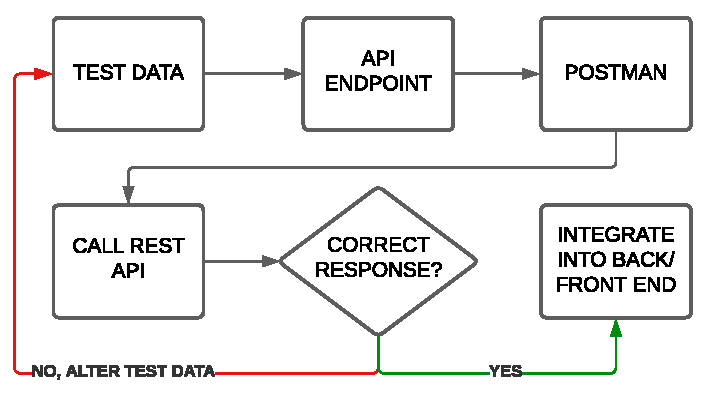
\includegraphics[width=370px]{figures/postman-testing.pdf}
  \caption{Postman - Testing external APIs}
  \label{fig:postman-external}
\end{figure}

\clearpage
\section{Chrome/React Developer Tools}
\label{testing:chrome-dev}

The Chrome/React Developer Tools were also used to test the front end during development. The debugger was used to ensure that the JavaScript was running correctly and that the data was being passed correctly between the front and back end. Logs and breakpoints were also used to track the flow of data through the front end, ensuring that the state was being updated correctly and that the correct data was being passed to the components \see{fig:dev-tools}.

\begin{figure}[!ht]
  \centering
  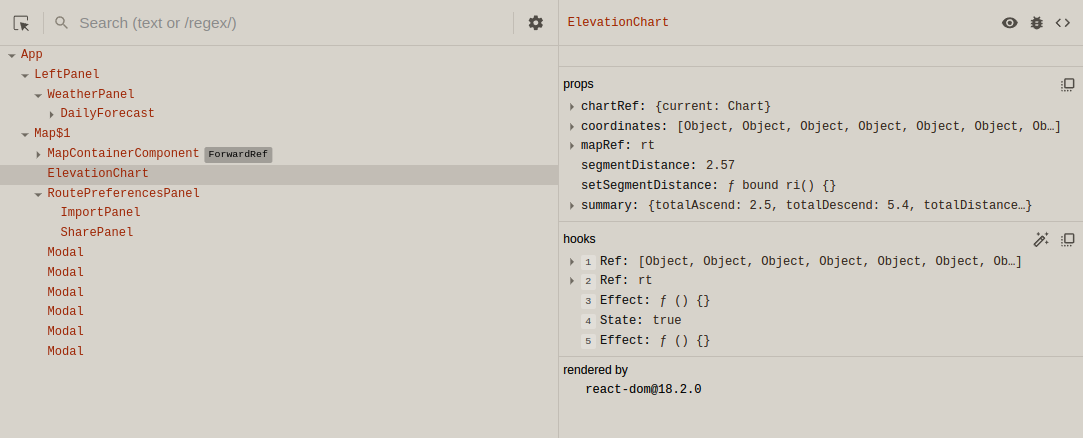
\includegraphics[width=370px]{figures/chrome-dev-tools-react.png}
  \caption{Chrome/React Developer Tools}
  \label{fig:dev-tools}
\end{figure}

\section{Conclusion}
\label{testing:conclusion}

A multi-faceted approach to testing was used where all core logic was tested to ensure the reliability of the final product. Testing enabled effective software development, ensuring all deadlines were met and that the artefact was delivered to a high standard.